%------------------------------------------------------------------------------------------------------------------------------------
\subsubsection*{The dynamic OOBN model}\label{Section:DaimlerDynamic}
%------------------------------------------------------------------------------------------------------------------------------------

The above described static OOBN is able to detect a manoeuvre $0.6$ seconds before execution. As detailed in Deliverable 1.2 \cite{Fer14b}, the goal is to enhance the prediction of manoeuvre recognition to at least $1-2$ seconds before the actual lane marking crossing. Moreover, this early detection of the manoeuvre should not be at the expense of the prediction accuracy. As specified in Deliverable 1.2 \cite{Fer14b}, the area under the ROC curve (AUC) should be greater than $0.96$ for $1$ second and greater than $0.9$ for $2$ seconds.

Figure \ref{Figure:daimlerTPlot} shows an example of the performance and limitations of the current static OOBN model. Two randomly selected manoeuvre sequences, namely seq1 (OBJ-CutOut) and seq2 (OBJ-CutIn), are considered.

\begin{figure}[ht!]
\begin{center}
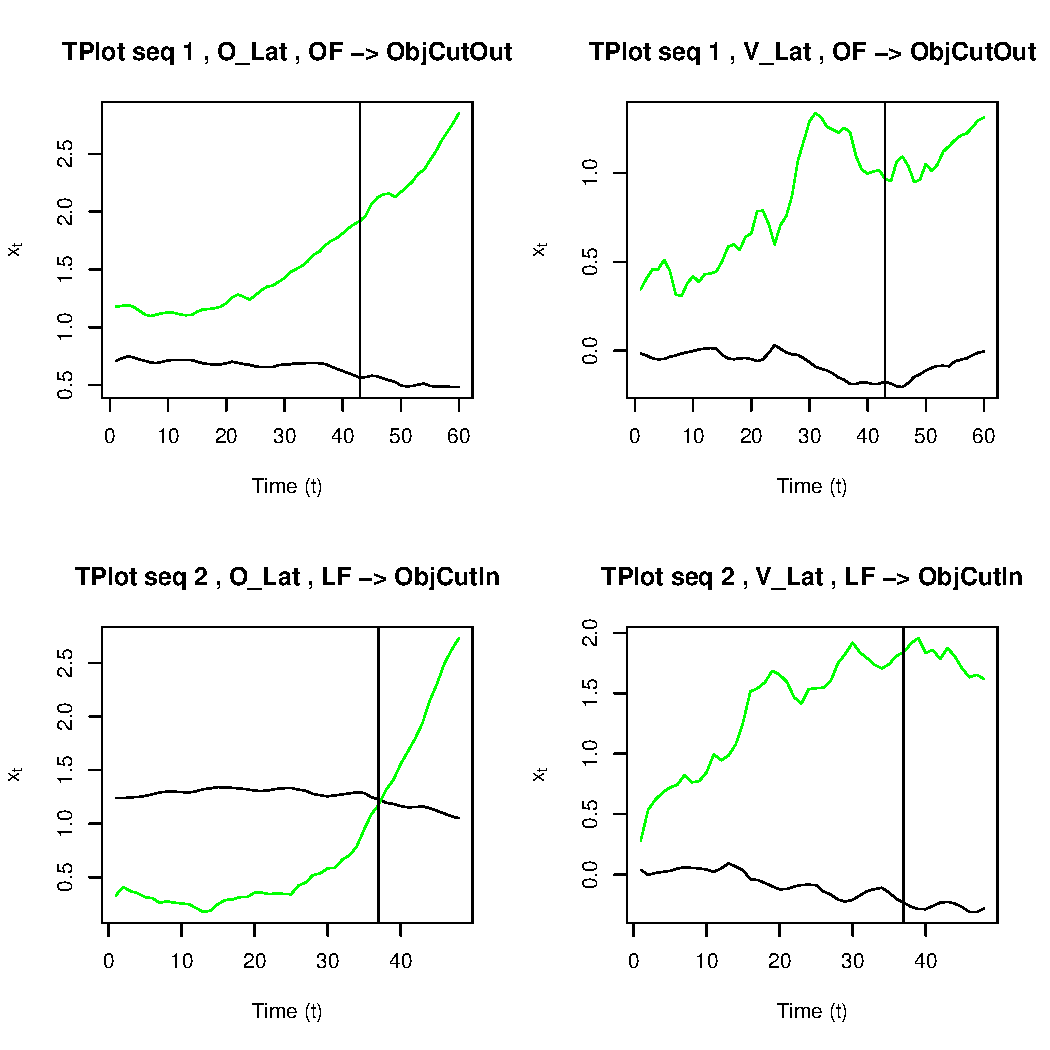
\includegraphics[scale=0.65]{./figures/DaimlerLE_EGO_L_LE_OBJ_R_OBJCut.pdf}
\caption{\label{Figure:daimlerTPlot}Time plots of the lateral offset (O\_Lat) and the lateral velocity (V\_Lat) for EGO (black curves) and OBJ (green curves) in two randomly selected sequences of an ObjCutOut (seq 1) and an ObjCutIn (seq 2). The x-axis corresponds to the different time-steps. On the left-hand side figures, the y-axis corresponds to the O\_Lat, while on the right-hand side figures, it corresponds to the V\_Lat.}
\end{center}
\end{figure}

For each sequence, we plot the evolution of different time-steps for lateral offset (O\_Lat) and lateral velocity (V\_Lat) to a lane marking. In each figure, the vertical black bar indicates the moment in which the manoeuvre has been correctly detected by the current static OOBN model. The manoeuvre is finished at the end of the series, which coincides with the actual moment of changed lane. The black curve corresponds to the O\_Lat and V\_Lat values of the EGO car, which is either following OBJ vehicle in the uppermost figures (OF) or following the lane (LF) in the lowermost figures. The green curve corresponds to the O\_Lat and V\_Lat  values of the OBJ car performing the OBJ-CutOut/OBJ-CutIn manoeuvres. 

As expected, for both OF and LF, the lateral offset of EGO is almost constant all the time (left-hand side figures), and its lateral velocity fluctuates around zero (right-hand figures), because in the two considered manoeuvre sequences EGO car is just driving inside its lane. However, we can easily see a different behaviour for the OBJ car (green curves): First, the lateral offset of OBJ steadily increases (left-hand side figures), which clearly indicates that the OBJ car is leaving its current lane in both manoeuvres. Second, the lateral velocity of OBJ is also much higher (right-hand side figures), indicating a lateral movement of OBJ. 

Although the manoeuvre is clearly identified before it completes in both considered sequences, it is desired to predict it \textit{further} in advance. Looking at the evolution of lateral offset and velocity in Figure \ref{Figure:daimlerTPlot}, we could argue that the detection of the manoeuvre can be performed earlier (i.e., when the lateral offset and lateral velocity starts to increase more dramatically and consistently for \textit{several} time-steps). This is one of the basic pieces of evidence that motivates the development of the dynamic version of the static OOBN model \cite{Weidl2014}. 

\begin{figure}[ht!]
  \centering
    \begin{tabular}{cc}
    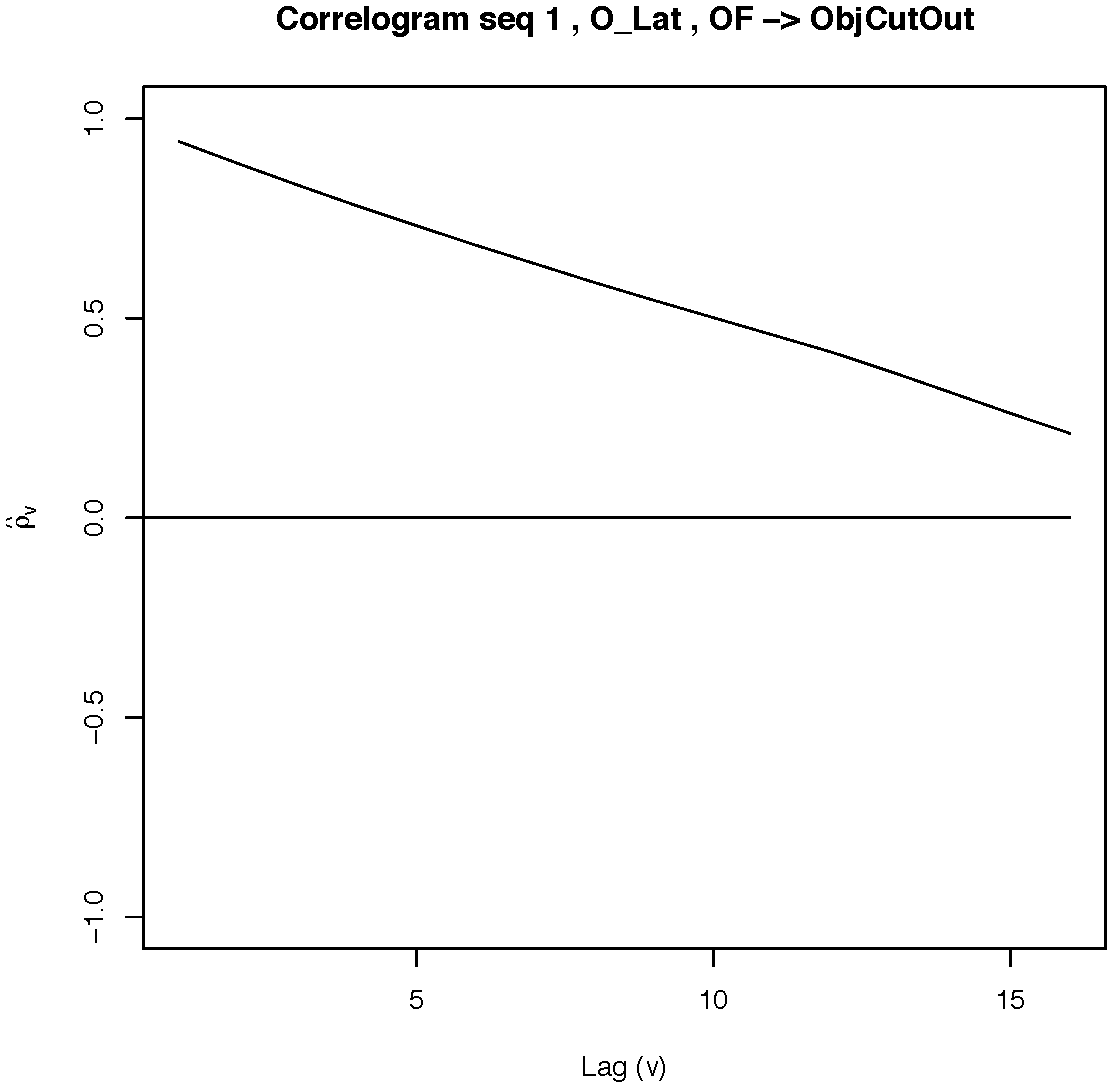
\includegraphics[width=60mm]{figures/DaimlerCorrOBJ_R15Offs.pdf}&
    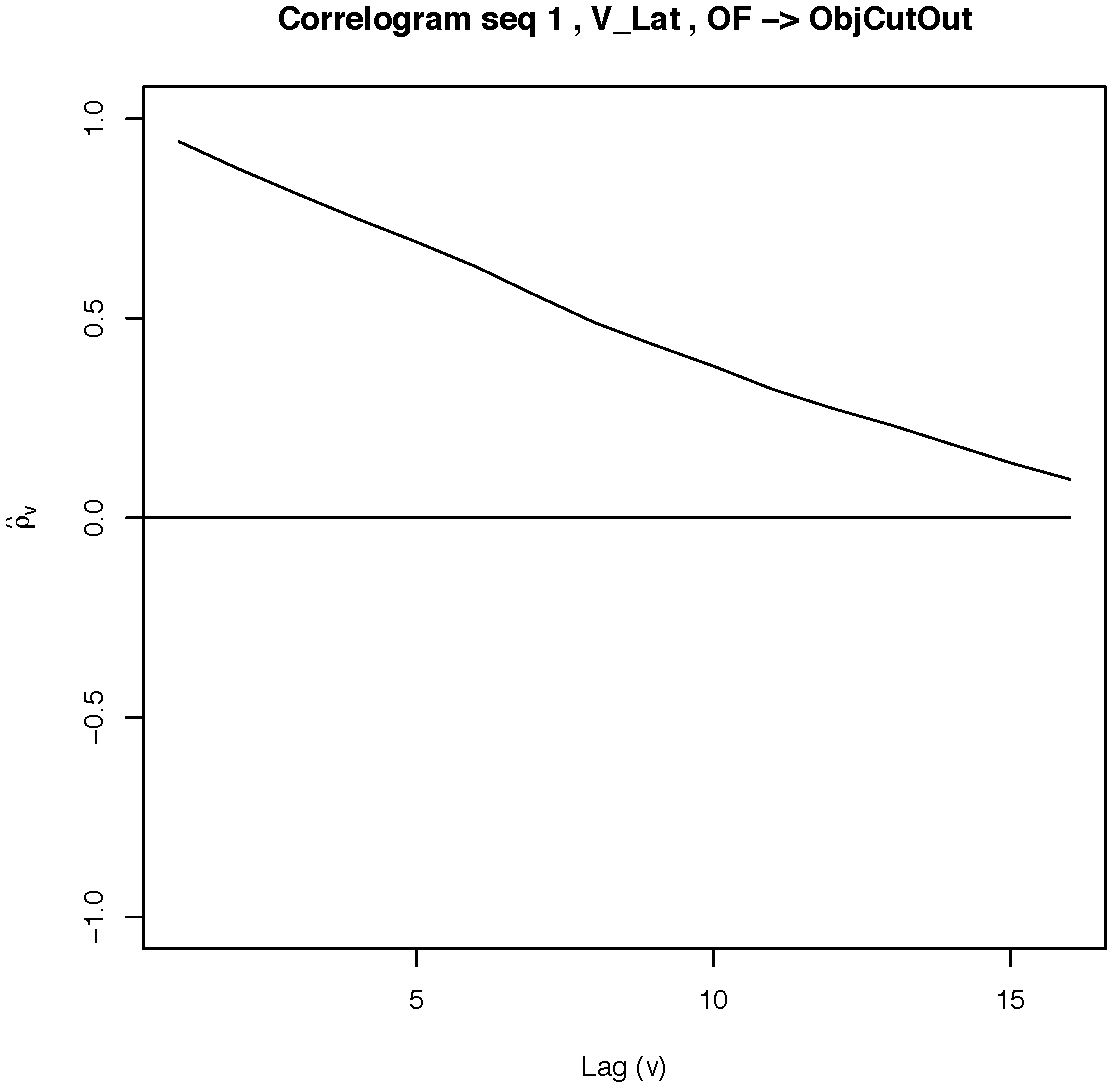
\includegraphics[width=60mm]{figures/DaimlerCorrOBJ_R15Vel.pdf}\\
  \end{tabular}
    \caption{\label{Figure:daimlerCorrel}Correlograms for lateral offset (O\_Lat) and the lateral velocity (V\_Lat). The x-axis represents the lag $v$ or time difference, and the y-axis represents the sample autocorrelation coefficient of lag $v$, denoted by $\hat{\rho_v}$, i.e., the correlation between variables at times $t$ and $t+v$ (see Section \ref{SubSection:CorrelogramsAndPartialCorrelograms} for more details).}
\end{figure}

In any case, let us note, that the prediction horizon for manoeuvre recognition is going to be limited in order to avoid false positives (i.e. recognizing a lane change manoeuvre when the driver was just performing some random lateral movement).  In case of a false positive, such as an erroneously OBJ-CutIn for instance, the adaptive cruise control would react with an unnecessary break, so they ought to be avoided. It is then required to find a good balance between the rate of false positives and false negatives. 

An additional piece of evidence that motivates the use of dynamic models appears when we look at the sample correlograms for lateral velocity and offset (that is, the correlation of the data with lagged values of themselves) plotted in Figure \ref{Figure:daimlerCorrel}. There we can see a strong temporal dependency (the correlation coefficients are high) for the two variables when we consider a \textit{small} number of time-steps between the temporal observations. Hence, the use of a dynamic model to make predictions about the evolution of the lateral velocity and lateral offset in a near future seems to be reasonable according to this analysis. Moreover, our main assumption is that the use of dynamic Bayesian network models (see Section \ref{SubSection:DBNs}) will allow us to build a more accurate, reliable, and robust system for manoeuvre recognition. 

As previously explained, the dynamic extension involves copies of the static OOBN for different number of time-steps in the time window. Figure \ref{Figure:daimlerLEdyn} shows an example for the LE hypothesis, where the nodes for O\_LAT\_REAL and V\_LAT\_REAL are temporal clones defining the belief state between consecutive time-steps, and hence creating a first order Markov process. This model has been proposed in \cite{Weidl2014}\footnote{\cite{Weidl2014} is an AMIDST paper (but includes some results from work done before AMIDST).} by some of the AMIDST partners. The first order assumption is a standard assumption in this kind of models and helps to simplify the posterior inference and learning process. This assumption is supported by the data: if we build a partial correlogram as the ones plotted in Figure \ref{Figure:daimlerPartialCorrel}, we can see that this assumption seems reasonable, because the influence of the lateral offset at time $t-1$ on the lateral offset at time $t+1$ given the lateral offset at time $t$ is close to null (i.e., the value at $v=2$ for the lag is close to null in Figure \ref{Figure:daimlerPartialCorrel}). Note that the same reasoning applies also to the lateral velocity.

\begin{figure}[ht!]
\begin{center}
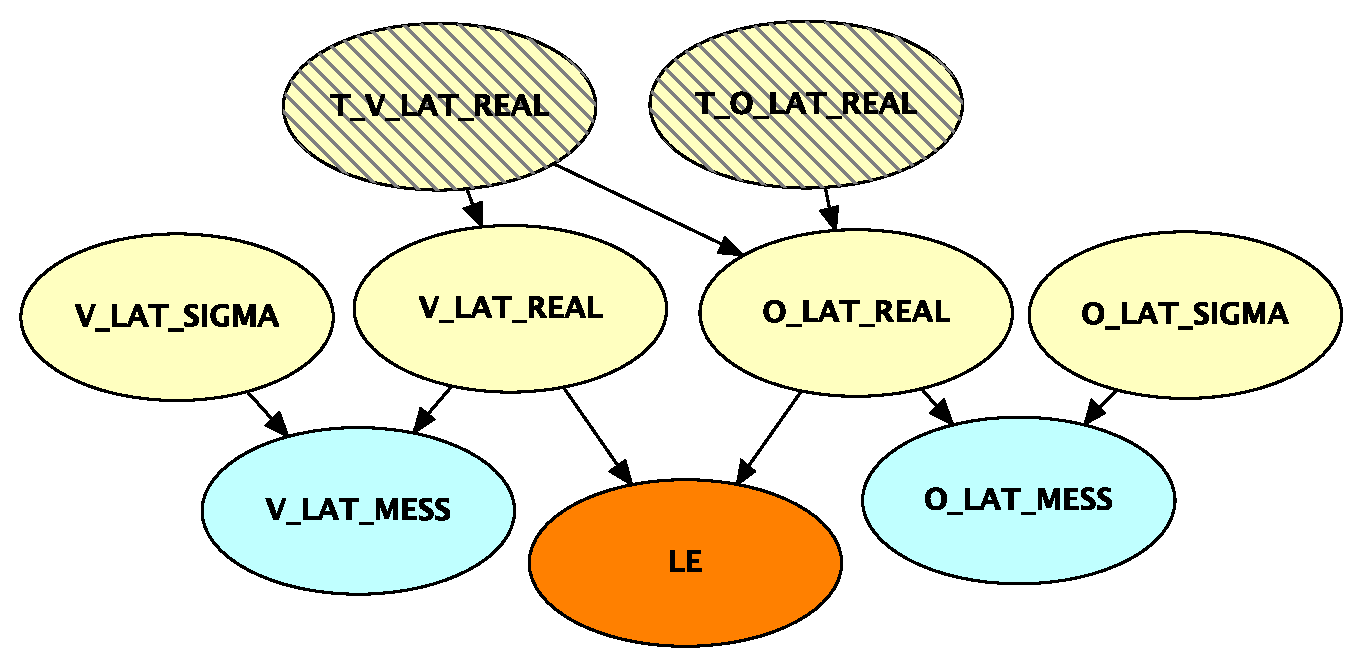
\includegraphics[scale=0.48]{./figures/DaimlerLEdyn}
\end{center}
\caption{\label{Figure:daimlerLEdyn}Daimler dynamic OOBN fragment for LE hypothesis.}
\end{figure}

\begin{figure}[ht!]
  \centering
    \begin{tabular}{cc}
        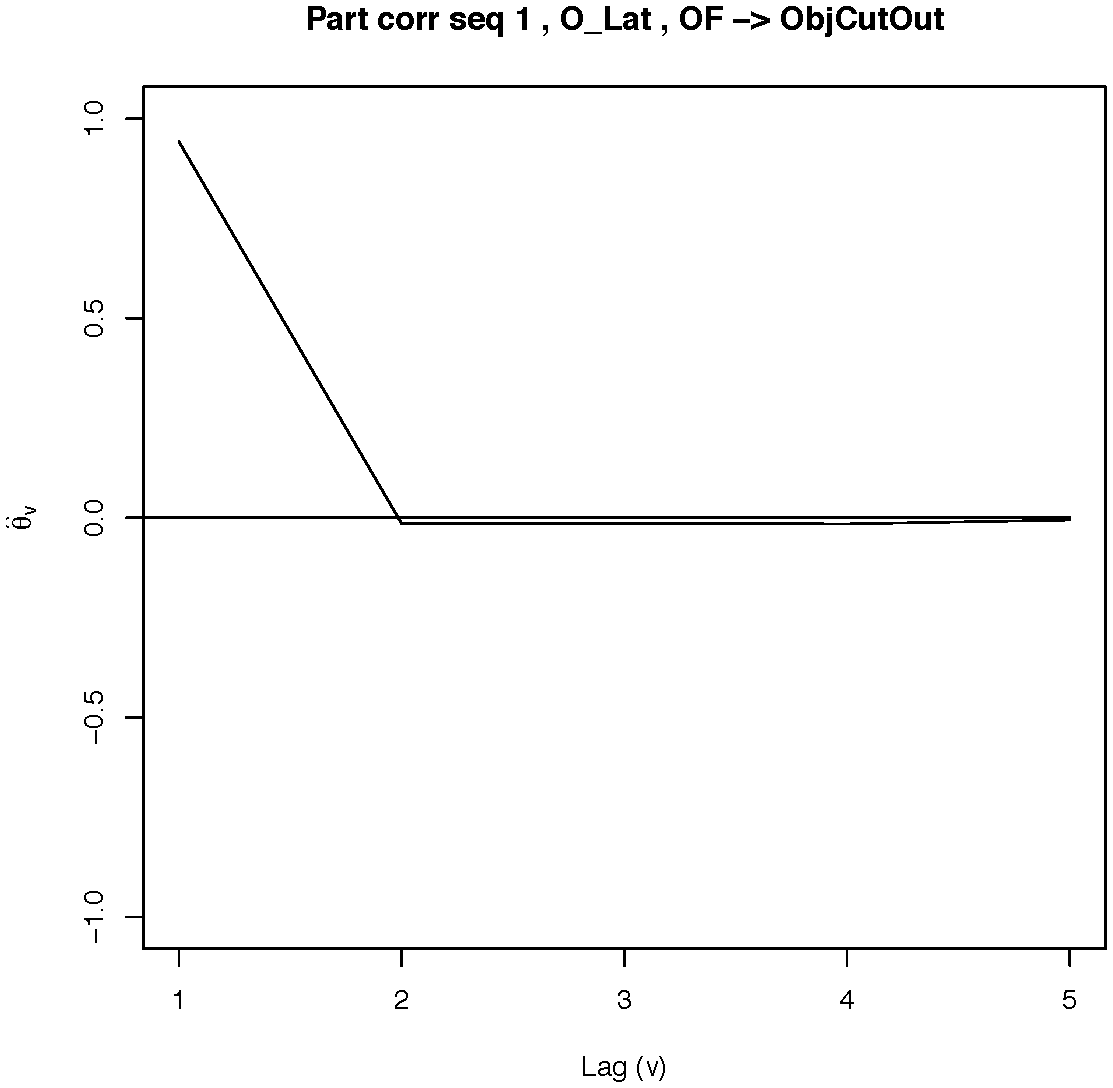
\includegraphics[width=60mm]{figures/DaimlerPcorrOBJ_R5Offs.pdf}&
    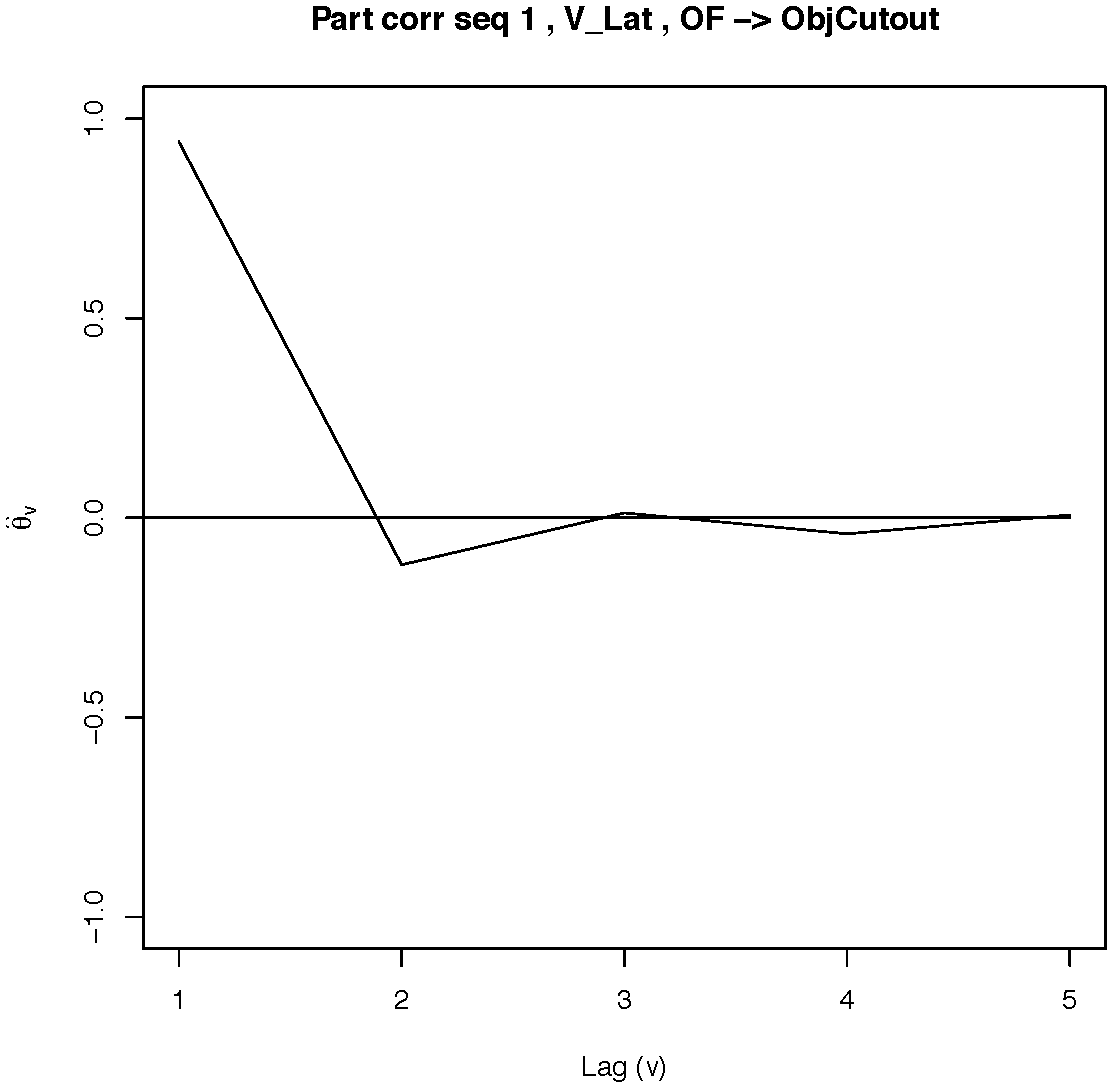
\includegraphics[width=60mm]{figures/DaimlerPcorrOBJ_R5Vel.pdf}\\
  \end{tabular}
    \caption{\label{Figure:daimlerPartialCorrel}Partial correlograms for lateral offset (O\_Lat) and the lateral velocity (V\_Lat). The x-axis represents the lag $v$ or time difference, and the y-axis represents the partial autocorrelation coefficient of lag $v$, denoted by $\ddot{\theta_v}$, i.e., the correlation between variables at times $t$ and $t+v$ after having removed the common linear effect of the data in between (see Section \ref{SubSection:CorrelogramsAndPartialCorrelograms} for more details).}
\end{figure}

As described in \cite{Weidl2014}, the proposed DBN aims to incorporate the trend of change for the real values, where their physical relations are represented as causal dependencies between the time-steps $dt$. For instance, in Figure \ref{Figure:daimlerLEdyn}, the transition function of O\_LAT\_REAL at time $t$, denoted as $O(t)$, is modelled as a Gaussian distribution. Its mean is affected by $O(t-1)$, and by V\_LAT\_REAL at time $t-1$, denoted as $V(t-1)$. Therefore, we have:

\begin{equation}
O(t) =O(t-1) +V(t-1)dt +\epsilon
\end{equation}

where $\epsilon$ denotes a white noise $\mathcal{N}(0,\sigma^2)$ which is assumed to be small. In order to corroborate the validity of this distributional assumption, we also analysed the hypothesis $O(t) - O(t-1) = \Delta O = V(t-1)dt +\epsilon$ on our data. Figure \ref{Figure:daimlerVvsOffs} shows the time and bivariate contour plots for $V(t-1)$ and $\Delta O$ for a randomly selected sequence (i.e., Seq 7) of an OBJ-CutOut manoeuvre. Both plots clearly corroborate that the assumption of a linear relationship with Gaussian noise might not be very far from reality.

The avid reader may have also noticed that these approaches do not take acceleration into account, i.e., they assume that velocity is constant (plus some white noise) at all times. From time plots corresponding to velocity in Figure \ref{Figure:daimlerTPlot}, we can easily observe that this is an unrealistic assumption. A more detailed analysis about the possible future inclusion of acceleration in the dynamic models is included below in Section \ref{subsubsection:daimlerfuture}, where future models are discussed.

\begin{figure}[ht!]
  \centering
  \setlength{\tabcolsep}{0.05pt}
  \renewcommand{\arraystretch}{0.02}
    \begin{tabular}{cc}
    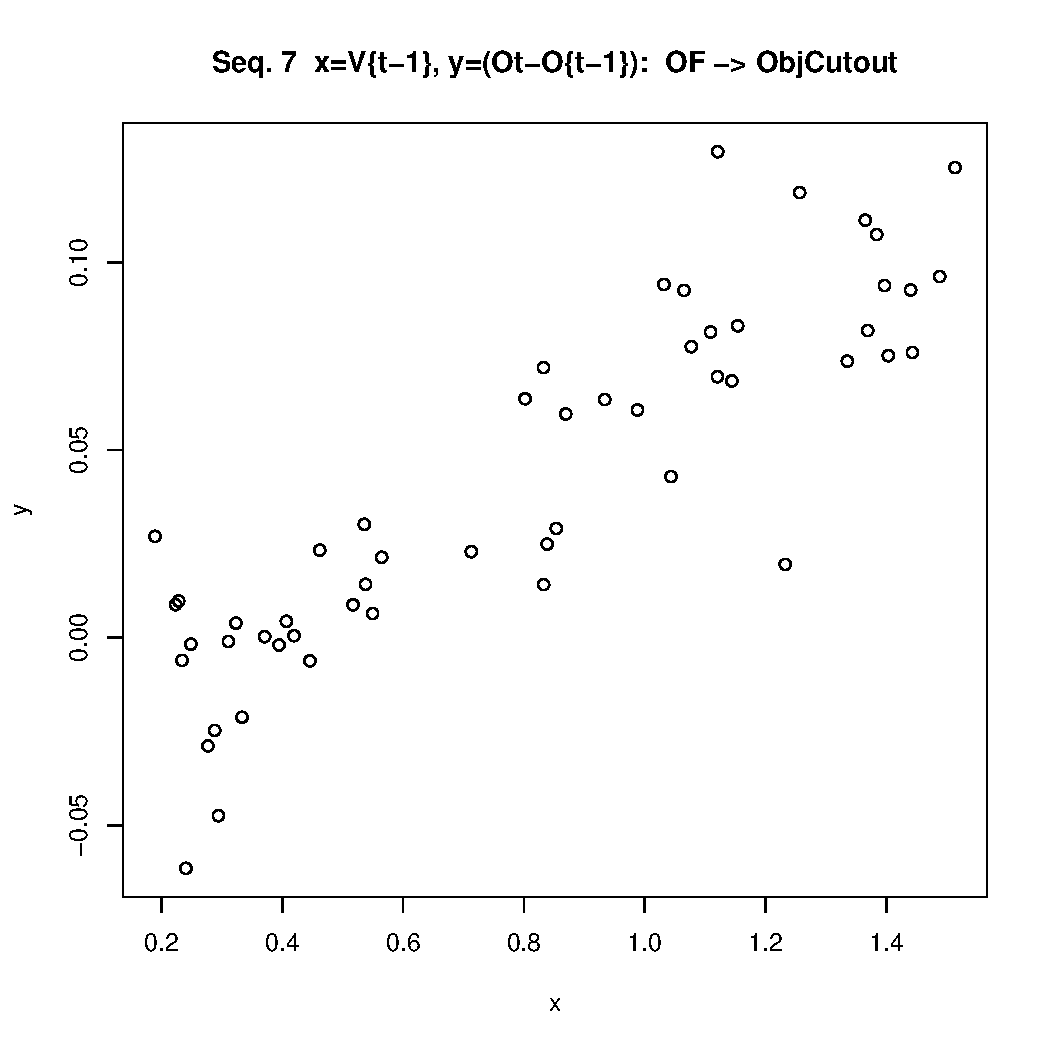
\includegraphics[width=60mm]{figures/DaimlerOBJplotSerie7.pdf}&
    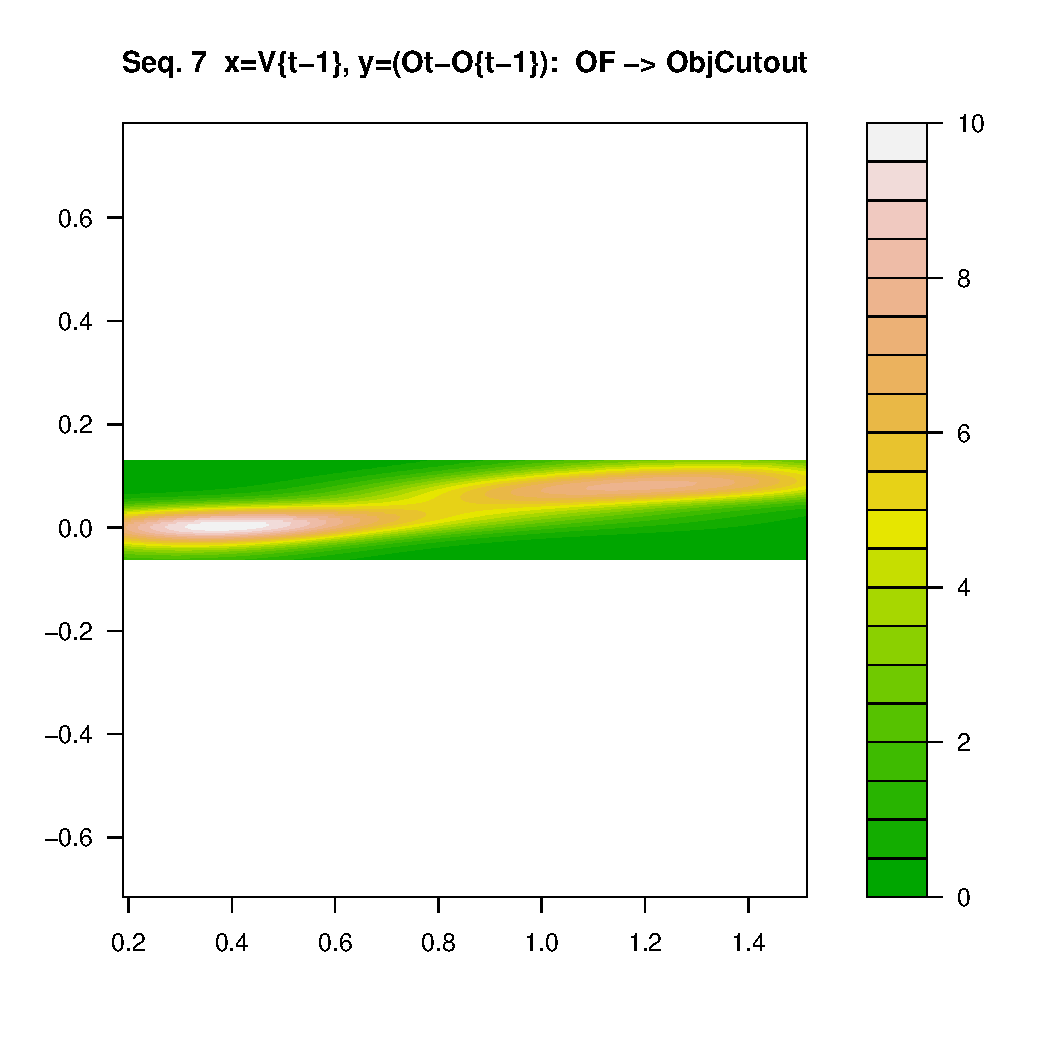
\includegraphics[width=60mm]{figures/DaimlerOBJcontourSerie7.pdf}\\
  \end{tabular}
      \caption{ \label{Figure:daimlerVvsOffs}Time and contour plots attesting the linear correlation between $V(t-1)$ versus $O(t) - O(t-1)$.}
\end{figure}

Finally, Figure \ref{Figure:daimlerLEdynGeneric} presents a rough overview of the final structure of the dynamic OOBN\footnote{Full details can not be provided for confidentiality reasons, but will be included in the confidential Deliverable 6.1.}. It illustrates how the temporal connection is only made on the top nodes (i.e., S\_REAL) involving the situation-features in consecutive time-steps\footnote{Although for the sake of clarity in the representation the sensor measurement structure is only shown for S\_REAL$_1$, this is identical for all sensor variables.}. The final event or manoeuvre prediction is then determined by the combination of all possible hypotheses ($Hypothesis_1, \ldots, Hypothesis_n$). There exist hypotheses at the top level that correspond to each of the sensor measurements, and then other different layers of hypotheses that combine the different outcomes till the final event, forming a polytree structure.

\begin{figure}[ht!]
\begin{center}
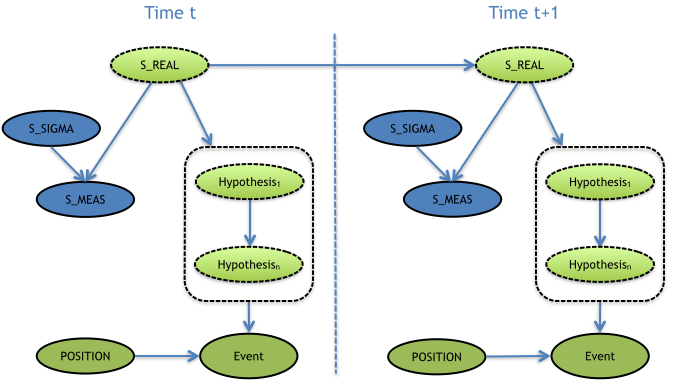
\includegraphics[scale=0.39]{./figures/DaimlerLEdynGeneric}
\end{center}
\caption{\label{Figure:daimlerLEdynGeneric}Daimler dynamic OOBN model with several hypotheses. Although for the sake of clarity in the representation the sensor measurement structure (i.e., S\_MEAS and S\_SIGMA) is only shown for S\_REAL$_1$, this is identical for all sensor variables. S\_REAL variables are plotted in green color to highlight that they are discretized, because otherwise we would have a model with continuous parents and discrete children.}
\end{figure}

Similarly to the static OOBN, if we modelled V\_LAT\_REAL and O\_LAT\_REAL as continuous variables, the conditional probability distribution of the LE hypotheses given the V\_LAT\_REAL and O\_LAT\_REAL variables would not fall in the conditional linear Gaussian family \cite{JensenNielsen2007}, because we would have discrete children with continuous parents. Once again, the pursued approach to deal with this problem is the discretization of the V\_LAT\_REAL and O\_LAT\_REAL variables. Hence, they are represented with a green color in Figure \ref{Figure:daimlerLEdynGeneric} and in all the more generic versions of it that will be included in Section \ref{daimlerAMIDSTModels}. Since the remaining continuous variables S\_MEAS and S\_SIGMA are always observed (i.e., their corresponding potentials simplify to numbers), all the inferences can be implemented only over discrete potentials.

%-------------------------------------------------------------------------------------------------------------------------------------------------------
\subsubsection{Earlier prediction of the need for a lane change based on relative dynamics}
%-------------------------------------------------------------------------------------------------------------------------------------------------------

Earlier prediction of manoeuvre intentions could be achieved before any development of the trend for lateral evidence has been observed. A first indication of possible lane change intention could be detected through the relative dynamics between one vehicle (e.g., EGO) and the vehicles in front of it on the same lane. For instance, if a vehicle is driving slowly in front of the EGO vehicle on the same lane, this may indicate a need for a lane change. In fact, in order to continue its safe driving, the EGO vehicle should either break and reduce its speed to the speed of the vehicle in front, or alternatively, change to the adjacent lane, if the neighbour lane is free and no other vehicle is approaching with a higher speed. 

A continued safe manoeuvre (of type ``lane follow'' or ``lane change'') is modelled by estimating the time to collision (TTC) with a vehicle in front (on the same lane) or eventually with an approaching vehicle (on the neighbour lane). For a safe manoeuvre, TTC should be higher than $1$ second, either when the EGO vehicle wants to change to the neighbour lane or needs to break to ensure safe driving on the same lane. We assume that using this approach will further enhance the prediction horizon for manoeuvre recognition.

Similarly to the models described in Figure \ref{Figure:daimlerLEdyn}, the dynamic OOBN model, shown in Figure \ref{Figure:daimlerreldyn}, was defined with the hypothesis ``relative dynamics'' (REL\_DYN) \cite{SlavaThesis2014}. Due to confidentiality reasons, we can not give at this stage of the project further details about this model (full details will be given in the confidential Deliverable 6.1.).

 
\begin{figure}[ht!]
\begin{center}
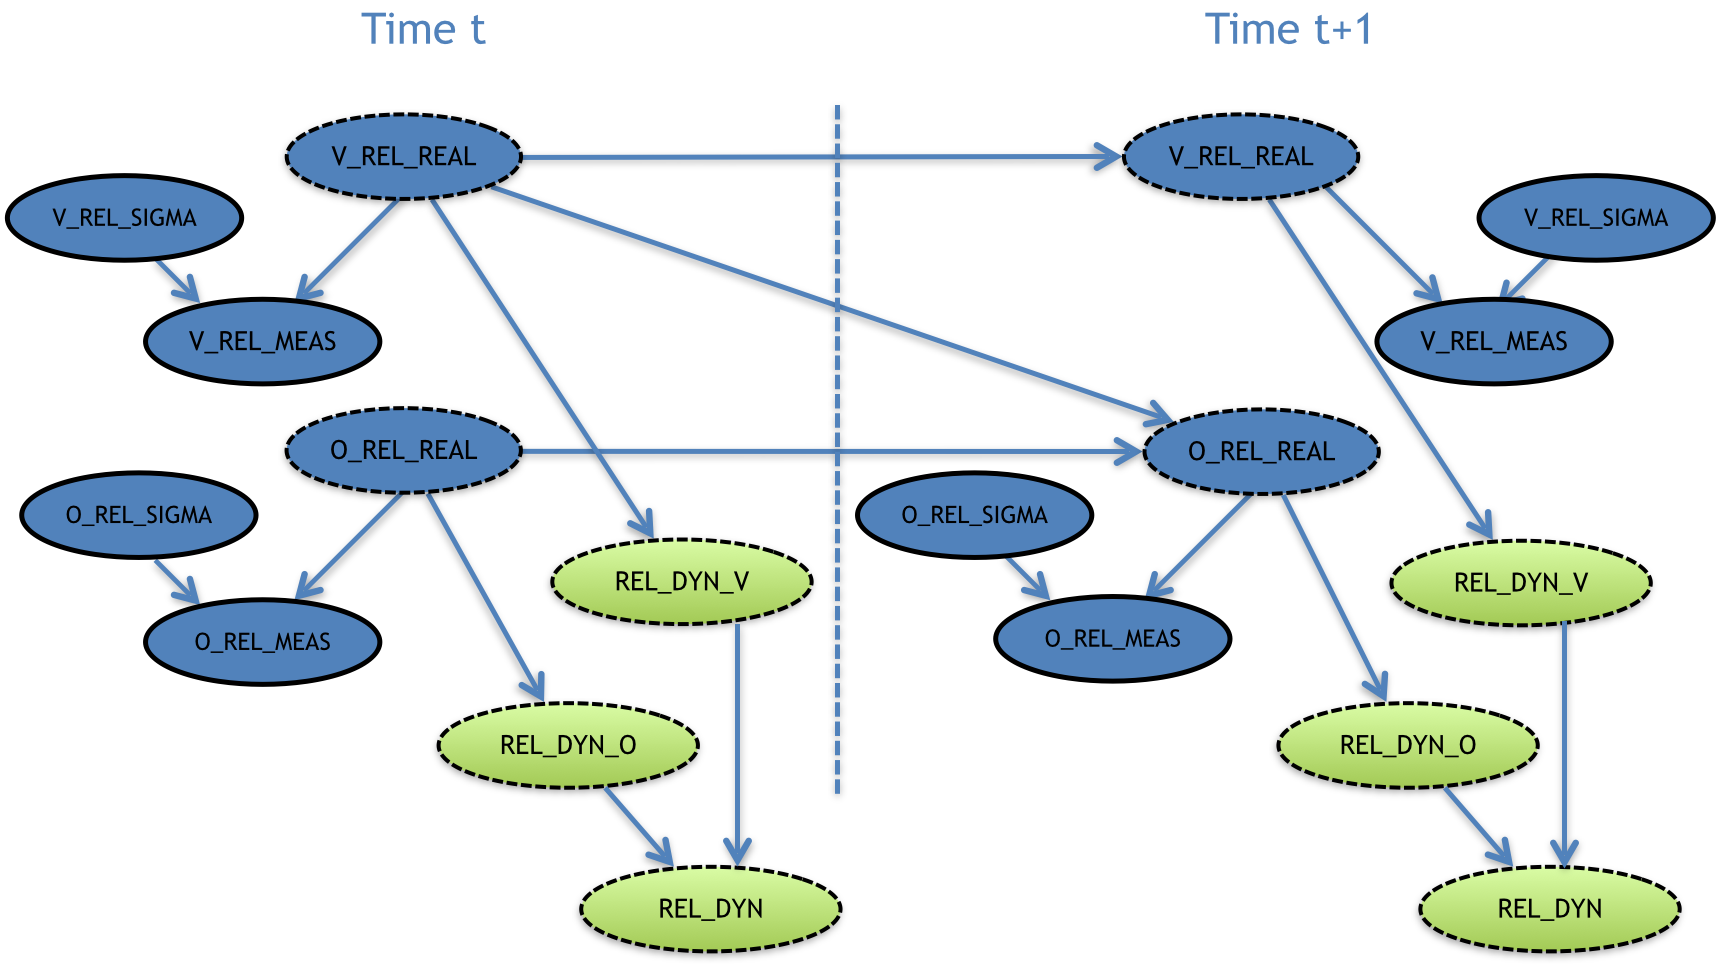
\includegraphics[scale=0.48]{./figures/Daimlerreldyn.png}
\end{center}
\caption{\label{Figure:daimlerreldyn}Daimler dynamic OOBN model with relative dynamics \cite{SlavaThesis2014}. V\_REL\_REAL and O\_REL\_REAL refer to the relative velocity and relative distance between the EGO and the car in front, respectively. The other variables with \_MEAS and \_SIGMA suffixes refer to the measured values and the uncertainty of the measurements, respectively, as commented in the previous section for other sensor readings.}
\end{figure}

%-------------------------------------------------------------------------------------------------------------------------------------------------------
\subsubsection{Discussion and future models}\label{subsubsection:daimlerfuture}
%-------------------------------------------------------------------------------------------------------------------------------------------------------

The above included proposals are preliminary models designed in line with the expert knowledge facilitated by Daimler. They all try to balance a good level of expressiveness and efficiency during inference. However, in any case, they should only be seen as first proposals that might be modified/adapted in the future if they do not meet the efficiency and accuracy targets specified in the requirements \cite{Fer14}. In addition, one thing to take into account is the time and space complexity of models. This will most likely induce changes to the initial structures outlined above.

For application scenario 1 (see Section \ref{Section:Daimler:EarlyRecognition}), we envision, for example, the possibility of considering not only the temporal dependences between consecutive time-steps for the sensor measurements but also, or instead, consider the temporal links between hypotheses at consecutive time-steps (i.e., adding in Figure \ref{Figure:daimlerLEdynGeneric} temporal links between hypotheses nodes at different time-steps). It seems natural, for instance, that the probability of the EGO lateral evidence would be higher given its lateral evidence at the previous time-step. The same applies for the remaining hypotheses, such as TRAJ, OCCGRID, and the final hypothesis or event that identifies the type of manoeuvre. However, adding these type of dependences would greatly increase the complexity of inference in the resulting dynamic OOBN, because the total number of dependencies will be much higher over time. As described in D1.2 \cite{Fer14}, models in this case are subject to very strong constraints in terms of computational efficiency, so we should be very cautions at this respect. 

Another possible extension is to consider an extra hidden variable to model the acceleration in the dynamic OOBN model. We believe that assuming that lateral velocity varies according to a constant acceleration can lead to inaccuracies. Figure \ref{Figure:daimlerVel} (a) shows the behaviour of lateral velocity (V\_Lat) for a randomly selected sequence which corresponds to an EGO-CutIn manoeuvre. At the beginning of the sequence, acceleration is close to zero, however, approximately between time-steps 30 and 50, a higher acceleration value should be taken into account.

\begin{figure}[ht!]
  \centering
  \setlength{\tabcolsep}{0.05pt}
  \renewcommand{\arraystretch}{0.02}
    \begin{tabular}{cc}
    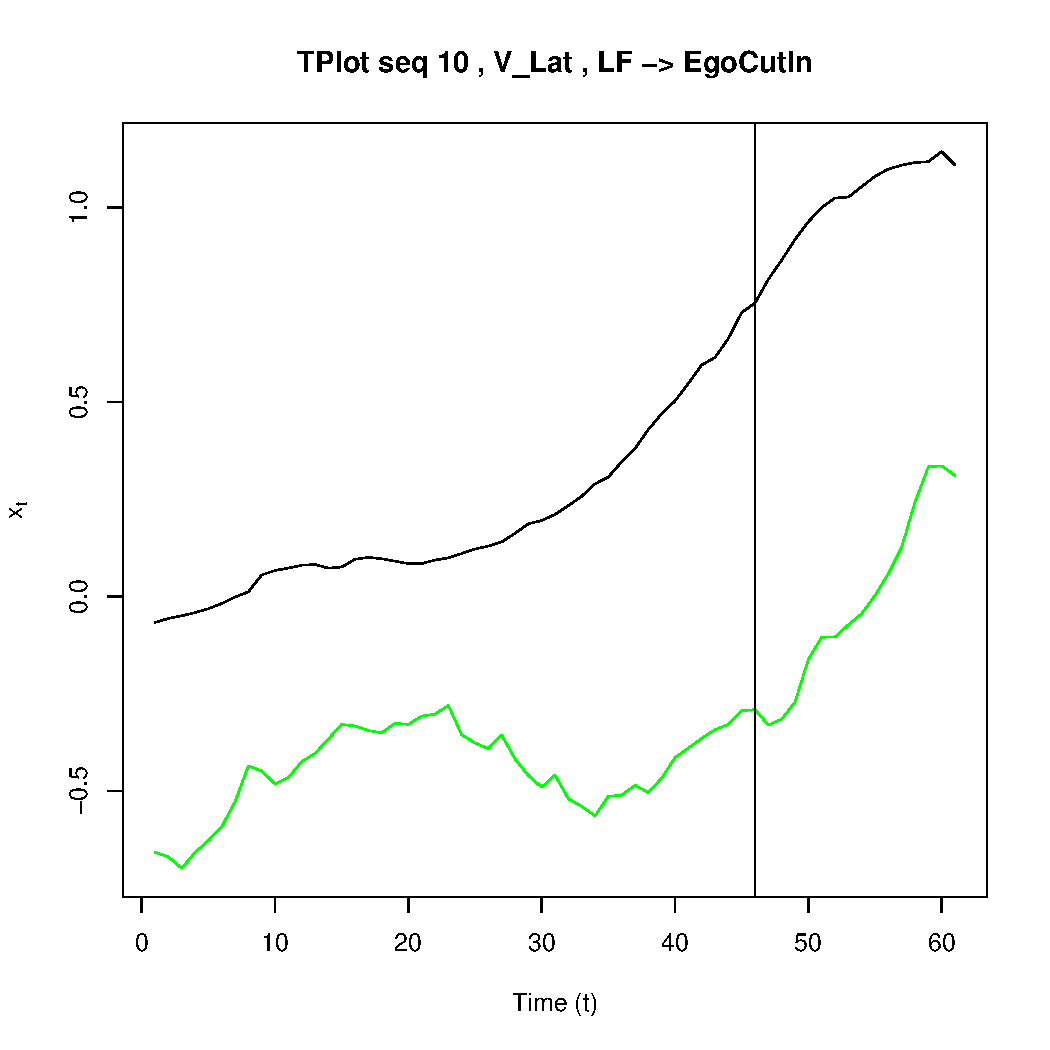
\includegraphics[width=60mm]{figures/DaimlerLE_EGO_L_LE_OBJ_R_EGOCutInVel.pdf}&
    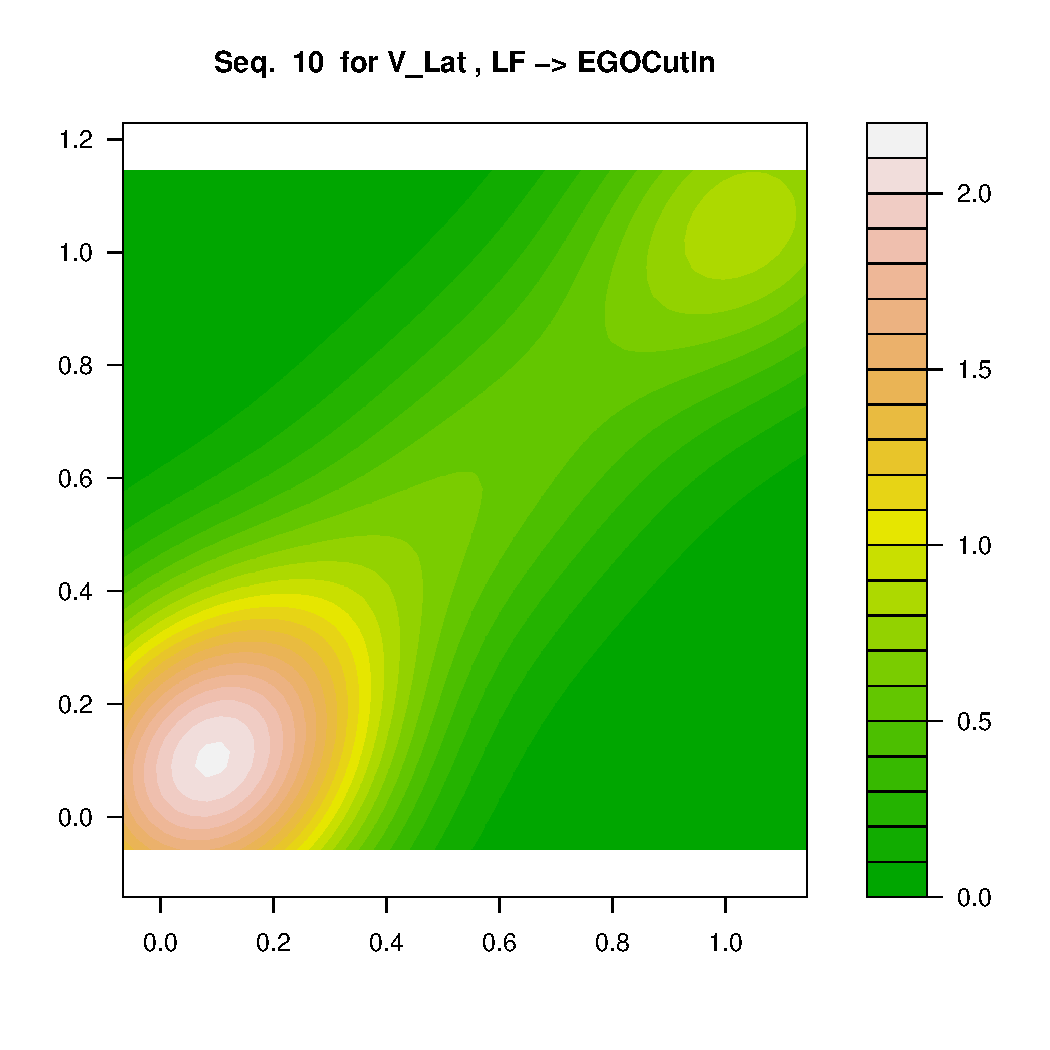
\includegraphics[width=60mm]{figures/DaimlerBivariate_temporal_analysisEGO_LVel.pdf}\\
  \end{tabular}
      \caption{ \label{Figure:daimlerVel}Time and contour plots for $V(t)$ versus $V(t-1)$ showing that modelling the acceleration should be considered to capture the variations in the data.}
\end{figure}

Moreover, the contour plot on Figure \ref{Figure:daimlerVel} (b) shows a large density of points for low and high $V$ values (i.e., where the acceleration is constant), but just isolated points in between. Hence, we think that the dynamic model could benefit from an extra hidden variable to represent acceleration (A\_Lat) as displayed in Figure \ref{Figure:tempDynAccel}. 


\begin{figure}[ht!]
\begin{center}
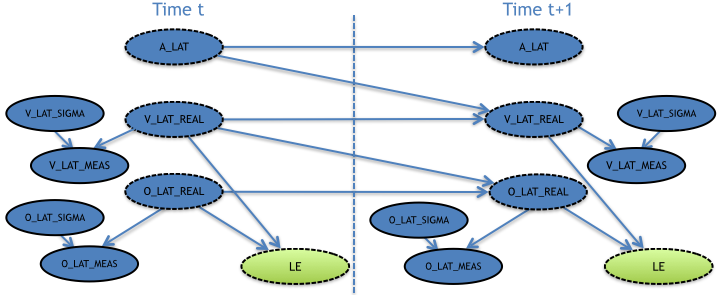
\includegraphics[scale=0.48]{./figures/DaimlertempDynAccel}
\end{center}
\caption{\label{Figure:tempDynAccel}Daimler dynamic OOBN fragment for the LE hypothesis with a hidden node for acceleration (A\_Lat).}
\end{figure}


The following equation would be then considered for velocity at consecutive time-steps:

\begin{equation}
V(t) =V(t-1) +A(t-1)dt +\epsilon
\end{equation}

\noindent where $A(t-1)$ denotes the acceleration at time-step $t-1$ and $\epsilon$ is a white noise. In this model, acceleration is assumed to be almost constant between two consecutive time-steps, i.e., $A(t) = A(t-1) + \epsilon$. 


